%-----------------------------------------------------------------------------
%
%               Template for sigplanconf LaTeX Class
%
% Name:         sigplanconf-template.tex
%
% Purpose:      A template for sigplanconf.cls, which is a LaTeX 2e class
%               file for SIGPLAN conference proceedings.
%
% Guide:        Refer to "Author's Guide to the ACM SIGPLAN Class,"
%               sigplanconf-guide.pdf
%
% Author:       Paul C. Anagnostopoulos
%               Windfall Software
%               978 371-2316
%               paul@windfall.com
%
% Created:      15 February 2005
%
%-----------------------------------------------------------------------------


%\documentclass[preprint]{sigplanconf}
\documentclass[10pt]{sigplanconf}

% The following \documentclass options may be useful:
%
% 10pt          To set in 10-point type instead of 9-point.
% 11pt          To set in 11-point type instead of 9-point.
% authoryear    To obtain author/year citation style instead of numeric.

\usepackage{yfonts}
\usepackage{amsmath}
\usepackage{amsthm}
\usepackage{amssymb}
%\usepackage{mathpartir}
\usepackage{url}
\usepackage{graphics}
\usepackage{graphicx}
\usepackage{wasysym}
\usepackage{harmony}
\usepackage{marvosym}
\usepackage{multirow}
\usepackage[usenames,dvipsnames]{xcolor}
\usepackage[utopia]{mathdesign}

% ____________________________________________________________
% Listings Package Configuration
% \usepackage[scaled]{beramono}

%\renewcommand*\ttdefault{txtt}
\usepackage[T1]{fontenc}

% This Deep Tex Voodoo is from
%   <http://www.latex-community.org/forum/viewtopic.php?f=5&t=2072>
% It's purpose is to make \lstinline normal size, without affecting
% \lstinputlisting.  It seems to work but I have no idea how or why,
% and I rather hope never to learn.
%\makeatletter
%\lst@AddToHook{TextStyle}{\let\lst@basicstyle\ttfamily\normalsize}
%\makeatother

\begin{document}

\conferenceinfo{SIGBOVIK '16}{Pittsburgh, PA, USA}
\copyrightyear{2016}
\copyrightdata{}

\titlebanner{banner above paper title}        % These are ignored unless
\preprintfooter{short description of paper}   % 'preprint' option specified.

\title{
Which ITG Stepcharts are Turniest?
}
% \subtitle{\em The Randomly-Scoped Lambda Calculus}
% \subtitle{Subtitle Text, if any}

\authorinfo{Ben Blum}{}{bblum@cs.cmu.edu}

\maketitle

\begin{abstract}
	ITG is a popular dance game in which players step on arrows while listening to music. The arrow patterns, indicated by a {\em stepchart}, may range among any level of complexity and difficulty. Among the many factors contributing to a stepchart's difficulty is how much the player must turn from side to side.
	Other more obvious factors, such as raw speed, have been well studied in prior work. % TODO cite.
	This paper presents an analytic study of this {\em turniness} factor.
	We study the turniness of many existing stepcharts, and present a novel (but unsurprising) approach to automatically generating maximally (or minimally) turny charts.
	Among real-world songs, we find stepcharts with overall turniness ranging from 0\% to 81.33\% of the theoretical maximum.


\end{abstract}

\category{D.D.R.}{Exercise and Fitness}{Arcade Dance Games}

\keywords
in, the, groove


\section{Introduction}

In 2005, Roxor Games, Inc. released {\em In The Groove}, a dance rhythm music video arcade fitness game, in which players control a protagonist using their feet to step on floor-mounted directional indicators. The protagonist, shown in Figure~\ref{fig:protagonist}, takes the form of any number of arrow-shaped directional receptacles, and must navigate a world of similarly-shaped obstacles (henceforth ``arrows'') by consuming them with the appropriate receptacle.
Roxor Games, Inc. In The Groove (henceforth ``ITG'') is most commonly played using the ``cabinet'' form factor, shown in Figure~\ref{fig:cab}, which includes two large metal dance pads, each with four directional indicators (henceforth, also, ``arrows'').

The game includes a library of rhythmic audio accompaniment files (henceforth, ``songs''), each of which is associated with one or more fixed patterns of arrows (henceforth, ``stepcharts''). These charts are often, but not always, synchronized to the beat of the song.
During gameplay, the stepcharts appear on screen and scroll towards the protagonist avatar at a rate either fixed or variable (henceforth, ``BPM'').
When the position of an arrow in the chart coincides with the avatar, the player must actuate the arrow of the corresponding direction.
The game will judge the player's timing accuracy, and penalize or reward them accordingly with scores and life bar fill.
A ``Fantastic'' judgement (as in Figure~\ref{fig:protagonist}) indicates a timing error not exceeding 15 milliseconds.
Other judgements include Excellent, Great, Decent, Way Off, and Miss.
As a visual assist to the player, notes are coloured according to their beat granularity:
\color{red}\Vier\color{black},
\color{Purple}\Vier$^3$\color{black},
\color{blue}\Acht\color{black},
\color{Purple}\Acht$^3$\color{black},
\color{LimeGreen}\Sech\color{black},
\color{Magenta}\Sech$^3$\color{black},
\color{Dandelion}\Zwdr\color{black}.


\begin{figure}[t]
	\begin{center}
	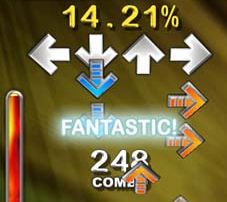
\includegraphics[width=0.2\textwidth]{protagonist.png}
	\end{center}
	\caption{ITG gameplay, including score indicator (top), protagonist avatar (mid), directional obstacles (low), and step judgement, life bar, and combo indicator (figure these out for yourself, I'm getting tired).}
	\label{fig:protagonist}
\end{figure}
\begin{figure}[t]
	\begin{center}
	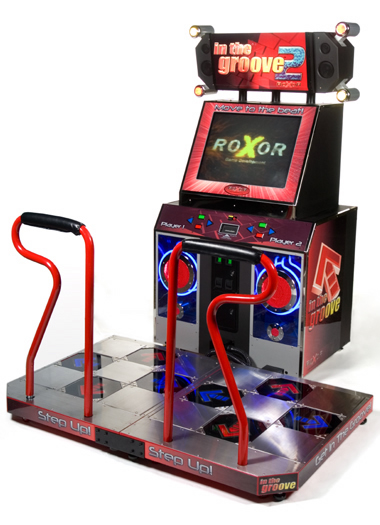
\includegraphics[width=0.18\textwidth]{itg2cabinet.jpg}
	\end{center}
	\caption{An ITG cab. RIP in peace, Roxor \cite{konami}.}
	\label{fig:cab}
\end{figure}

The game may be played in several modes, the most common supporting up to two (2) players, each operating their own protagonist using either the left or right set of four arrows.
This game mode may be played with or without the assist of a curved metal rod mounted behind the arrows (henceforth, ``bar''), as shown in Figure~\ref{fig:bengreg}.
In other game modes, a single player may operate up to all 8 of the arrows. When all 8 are used, the game mode is known as ``Doubles'', as shown in Figure~\ref{fig:jim}, and is often associated with excessive No-Barring, use of hands and knees to operate the arrows, and impressive facial hair.
In this body of work, we will focus exclusively on the Singles game mode, in which each player controls four arrows: one Up ($U$), one Down ($D$), one Left ($L$), and one Right ($R$). Without loss of generality, we further assume that only one player plays at a time, using exactly two feet at a time, and that she will shower immediately afterward.

\begin{figure}[t]
	\begin{center}
	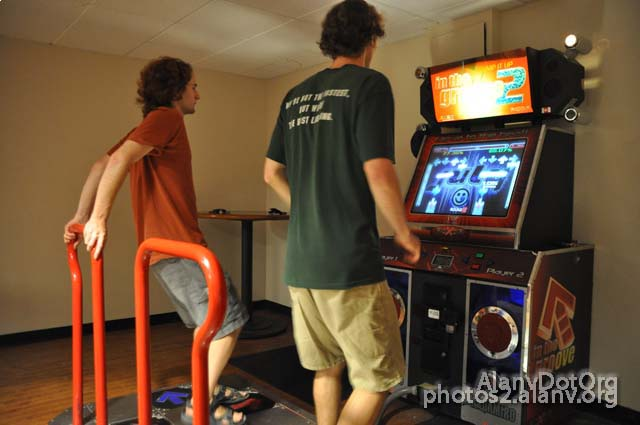
\includegraphics[width=0.48\textwidth]{bengreg.jpg}
	\end{center}
	\caption{ITG can be played ``Bar'' or ``No-Bar''. Bar players must wear sandals (like an idiot; who is that guy anyway?), while No-Barrers must always play on the right.}
	\label{fig:bengreg}
\end{figure}
\begin{figure}[t]
	\begin{center}
	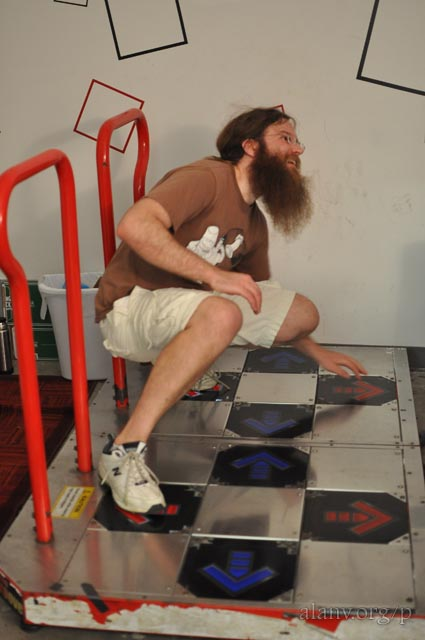
\includegraphics[width=0.2\textwidth]{jim.jpg}
	\end{center}
	\caption{Doubles play is beyond the scope of our work. It requires (or perhaps produces?) a magnificent beard.}
	\label{fig:jim}
\end{figure}

%%%%%%%%%%%%%%%%%%%%%%%%%%%%%%%%%%%%%%%%%%%%%%%%%%%%%%%%%%%%%%%%%%%%%%%%%%%%%%%%

\section{Properties of Stepcharts}

Being a game, one might assume that players find it fun to step the arrows in the indicated patterns, as opposed to, for example, stepping them in random unrelated patterns, or stepping off the pad entirely to go play Rocket League \cite{rocketleague}.
Accordingly, step authors take care to produce stepcharts with interesting patterns.
Typically, players step the arrows alternatingly with either foot.
Step authors can either reinforce this tendency, by maintaining that left and right arrow targets always receive arrows of different (even or odd) sequential parity;
or subvert it, forcing the player to step on the left arrow with their right foot (or v.v.).
The former pattern is called a {\em stream}, and the latter pattern a {\em crossover}. Crossovers are loved by some players (Figure~\ref{fig:bengreg}, left), and hated by others (Figure~\ref{fig:bengreg}, right).

Figure~\ref{fig:patterns} shows many common step patterns.
Among these, note especially the {\em lateral} ($LURLDR$), in which the player briefly faces backwards (left foot on $R$ and right foot on $L$), and the {\em spin} ($LURDLU$), in which, yeah, you get the picture.

\begin{figure}[t]
	\begin{center}
	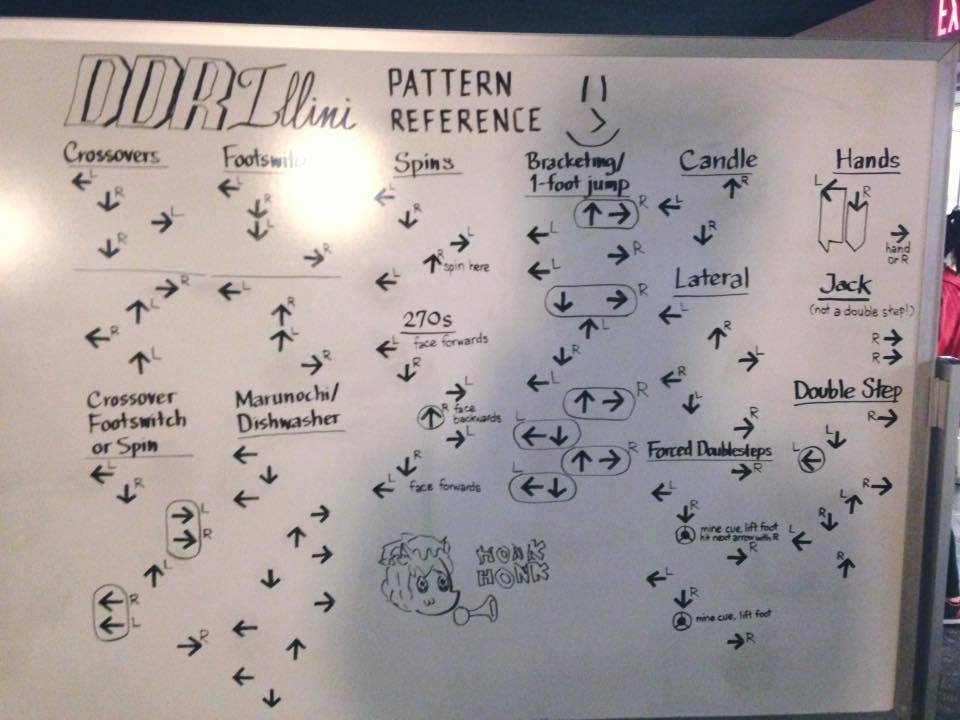
\includegraphics[width=0.48\textwidth]{patterns.jpg}
	\end{center}
	\caption{Common patterns \cite{patterns}. Honk honk!}
	\label{fig:patterns}
\end{figure}

\subsection{Difficulty}

Stepcharts are rated in difficulty on a scale from 1 to 20 ``feet'' \cite{simplylove}\footnote{
Other dance games \cite{konami}, which shall remain unnamed, feature wimpier stepcharts rated only up to 10, but as ITG players got better, they left those charts in the dust and began creating their own charts to challenge themselves with ridiculous difficulties. This paper's author plays ITG at the 13-14 level.}.
To date, difficulty is always judged by a human (typically the step author), and primarily reflects factors such as burstiness (footspeed), prolognedness of streams (stamina), and complexity of jumps, holds, and crossovers (technical).
These measures of difficulty have been well-studied in prior works \cite{callofthehound,dawgsinthehouse}.

\subsection{Facing}

Regardless of the presence of crossovers, all step patterns will keep the player {\em facing} one way or another, and most include sequences that will change the player's facing back and forth.
For example, when the player stands with left foot on $L$ and right foot on $U$, they are facing up-left, or $UL$. Standing on $D$ and $R$ also produces the same $UL$ facing, unless the player is crossed-over (left foot on $R$), in which case the facing is $DL$.
Table~\ref{tab:facing} shows all possibilities of facing using two feet on four arrows.
We exclude the possibility for both feet to be instantaneously on the same arrow (called a ``footswitch''), leaving this pattern to future work.

\begin{table}[h]
	\begin{center}
	\begin{tabular}{cc|cccc}
		& & \multicolumn{4}{c}{Right foot} \\
		& & $\leftarrow$ & $\downarrow$ & $\uparrow$ & $\rightarrow$ \\
		\hline
		\multirow{4}{*}{Left foot}
		%                 L   D   U   R
		& $\leftarrow$  & - & $UR$ & $UL$ & $U$ \\
		& $\downarrow$  & $DL$* & - & $L$ & $UL$ \\
		& $\uparrow$    & $DR$* & $R$ & - & $UR$ \\
		& $\rightarrow$ & $D\dagger$ & $DR$* & $DL$* & - \\

	\end{tabular}
	\end{center}
	\caption{Facing directions. ``Crossover'' facings are marked (*), and the ``lateral'' facing is marked ($\dagger$). Note the appealing diagonal symmetry.}
	\label{tab:facing}
\end{table}

\subsection{Turning}

A stepchart contains a {\em turn} when a sequence of steps changes the player's facing.

\newtheorem{definition}{Definition}
\begin{definition}[Turniness]
	The turniness $\mathcal{T}$ of a single step is the angular distance (measured in increments of $\pi/4$) which that step changes the facing compared to the facing from the previous two steps.

	The turniness $\mathcal{T}$ of a stream is the average of each step's turniness (excluding the first two for which it is undefined).
\end{definition}

Because only one foot may change at a time, it is easy to see that the maximum turniness of a single step is 2.
These steps always involve one foot moving entirely across the middle of the pad (from $U$ to $D$, from $L$ to $R$, etc).
By tradition, these are called {\em candle steps}, according to the imagery that if a candle were placed in the middle of the 4 arrows, this step would knock it over. I don't know why it couldn't be called a beer step instead, though.

{\bf Turning is exhausting.} Consider the three stream patterns shown in Figure~\ref{fig:stream}.
In the leftmost stream, the player must barely move her feet at all, never changing facing from $U$.
In the middle stream, the player faces largely $UR$, with brief $U$ facings ($\mathcal{T}=1$) as she moves between the $L$/$D$ and $U$/$R$ arrows.
Both of these streams are very easy to step without becoming fatigued.
However, the rightmost stream features many candle steps (or beer steps), changing facing from $UR$ to $UL$ and back in the span of a single measure.
ITG players hate this \cite{weirdtrick}!
However, note that even in this stream, not {\em all} of the steps have $\mathcal{T}=2$: the {\em average} turniness of this stream is only 4/3.

\begin{figure}[t]
	\begin{center}
	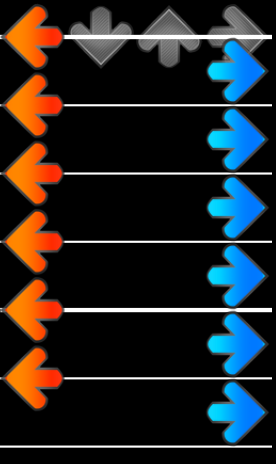
\includegraphics[width=0.15\textwidth]{tower.png}
	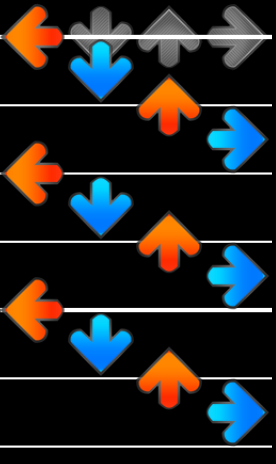
\includegraphics[width=0.15\textwidth]{staircase.png}
	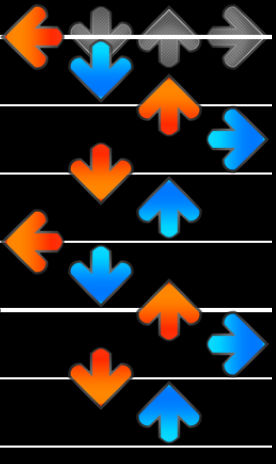
\includegraphics[width=0.15\textwidth]{twistystair.png}
	\end{center}
	\caption{Three streams of differing turniness.
	Note how the color-coding of the notes by beat aids to discern turniness at a glance: the right foot is always on blue, and it moves among 1, 2, or 3 different arrows respectively.}
	\label{fig:stream}
\end{figure}

We are interested in the following questions:
\begin{enumerate}
	\item What is the turniest possible stepchart?
	\item How is maximum turniness affected by various constraints to contain no crossovers/laterals/etc?
	\item How turny are real-world ITG charts?
\end{enumerate}

\section{Chart Synthesis}

We developed a program for exploring all possible step patterns using a little-known yet powerful computational technique \cite{bruteforce1,bruteforce2}.
This program computes the average turniness of every such pattern.
However, while some players enjoy any step pattern including spins \cite{alanv},
other players may prefer only crossovers and laterals in their charts,
while still others prefer charts completely vanilla.
Hence, our program is further capable of filtering patterns by 5 predicates:
\begin{itemize}
	\item All patterns allowed
	\item No spins
	\item No 270s
	\item No laterals
	\item No crossovers (vanilla)
\end{itemize}
Note that each predicate captures a strict subset of step patterns compared to the one above it (a lateral is a crossover, and so forth).
These predicates are implemented as shown in Figure~\ref{fig:eqn}.

\begin{figure*}
	\begin{eqnarray*}
		\mathsf{is\_xover}(\phi) &=& \phi \equiv DL \vee \phi \equiv DR \\
		\mathsf{is\_lat}(\phi) &=& \phi \equiv D \\
		\mathsf{is\_270}(\phi, \phi_1, \phi_2) &=& (\phi \equiv DR \wedge (\phi_1 \equiv DL \vee (\phi_1 \equiv D \wedge \phi_2 \equiv DL))) \vee \\
                                              & & (\phi \equiv DL \wedge (\phi_1 \equiv DR \vee (\phi_1 \equiv D \wedge \phi_2 \equiv DR))) \\
		\mathsf{is\_spin}(\phi, \phi_1, \phi_2, \phi_3) &=& (\phi \equiv R \vee \phi \equiv UR \vee \phi \equiv L \vee \phi \equiv UL) \wedge \mathsf{is\_270}(\phi_1, \phi_2, \phi_3)
	\end{eqnarray*}
	\caption{Formal definitions of crossovers, laterals, 270s, and spins. Each predicate takes as arguments the current facing $\phi$, and up to the three most recent previous facings, $\phi_1$, $\phi_2$, $\phi_3$.}
	\label{fig:eqn}
\end{figure*}

Deciding on how long of step sequences we should search for is a tradeoff between accuracy, in judging turniness in small fractions, and (drumroll...) exponential explosion.
To strike a balance we decided to experimentally measure turniness at a granularity of 1/8th, which requires searching for step sequences of length 18 (twice the denominator, plus 2 for the first 2 steps whose turniness is undefined).
Also, our program WLOG restricts streams to always start on the left foot, and never to start crossed over.
Figure~\ref{fig:graph} shows our results.
The highest data point clocks in at 40,609,780: there are over 40 million unique 18-step sequences, any patterns allowed, that have turniness 0.875.

We see that, with one exception, allowing each new type of step pattern increases the maximum possible turniness of the chart.
The exception is that 270s do not allow for any additional turniness over laterals, although they do allow for {\em more possible ways} to achieve maximum turniness.
Despite no additional turniness, this is crucial information for stepchart authors, as ITG players will (usually) get bored of any chart that simply repeats the same pattern over and over.

\begin{figure}[t]
	\begin{center}
	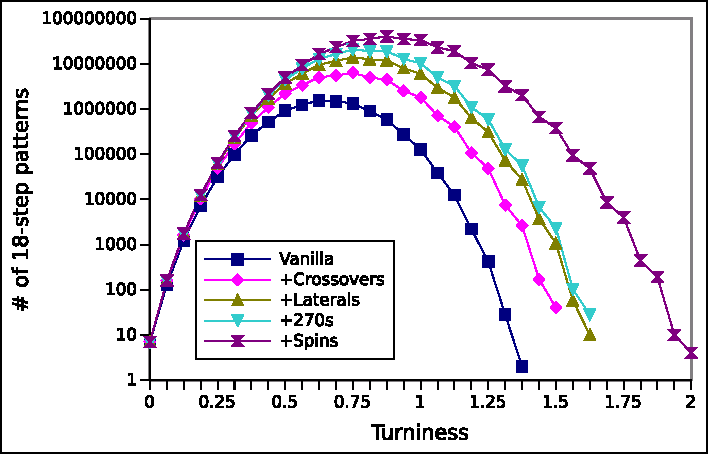
\includegraphics[width=0.48\textwidth]{turniness.pdf}
	\end{center}
	\caption{Distribution of unique step sequences among turninesses, classified by what types of step patterns are allowed in the chart.}
	\label{fig:graph}
\end{figure}

{\bf Maximum turniness!}
Now to the paper's titular question: what step sequences underlie those data points on the far right of each curve?
Though it would be tedious to transcribe them all into Stepmania's step editor \cite{stepmania}, we manually inspected many of them to select the most representative and/or photogenic ones from each category. We show these sequences in Figure~\ref{fig:sequences}.
These visualizations allow us to manually compute the true turniness of each sequence, imagining the core sequence repeated ad infinitum, freeing ourselves from the 1/8th granularity imposed by our experimental setup.
We find that the turniest crossovers have $\mathcal{T}=3/2$ and that the turniest laterals have $\mathcal{T}=8/5$.

The case of 270s is irregular: we found no 18-step sequence turnier than the turniest laterals, and most notably,
none of the sequences included a 270 step in the {\em middle} of the stream.
Figure~\ref{fig:sequences}(d) shows a stream with crossovers and laterals and no 270 step until the very last one.
To see why, imagine yourself on the pad here: the only possible 19th step that doesn't result in a spin is to step back on the same arrow your left foot is already on.
That step has $\mathcal{T}=0$, which would undo any potential turniness gained from going into the 270.
Nevertheless, 270s retain some real-world application, as demonstrated by \cite{utopia} which similarly employs a 270 as the very last step.

Perhaps predictably, pure spins make for the turniest possible chart. There are only two possible ways to candle every step; one's name is ``clockwise'', and you can guess the other.

{\bf Minimum turniness.}
Each of the 5 categories shares the same data point at $\mathcal{T}=0$: there are 7 possible streams that never turn at all. These are the 7 tower patterns $LULU$, $LRLR$, $LDLD$, $URUR$, $DRDR$, $UDUD$, and $DUDU$. We already showed the first of these in Figure~\ref{fig:stream}, left. For further treatment of minimally turny charts, we refer the reader to \cite{deltamax}.

\begin{figure*}[t]
	\begin{center}
	\begin{tabular}{ccccc}
		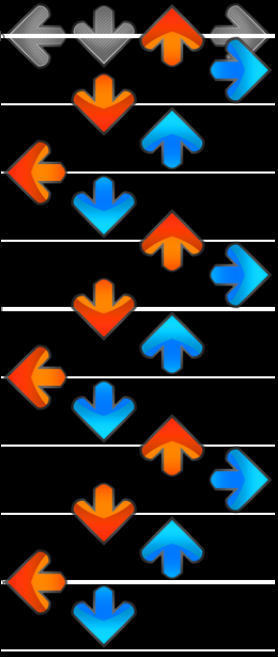
\includegraphics[width=0.17\textwidth]{result-1-3-vanilla.png} &
		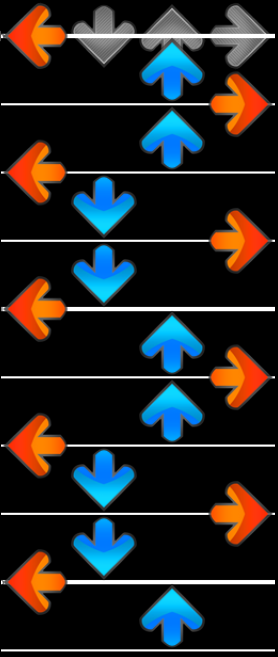
\includegraphics[width=0.17\textwidth]{result-1-5-xover.png} &
		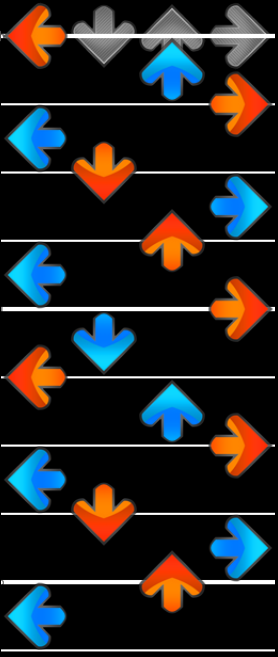
\includegraphics[width=0.17\textwidth]{result-1-6-lats.png} &
		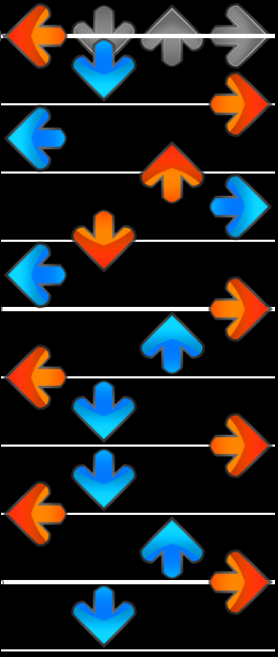
\includegraphics[width=0.17\textwidth]{result-irregular-270.png} &
		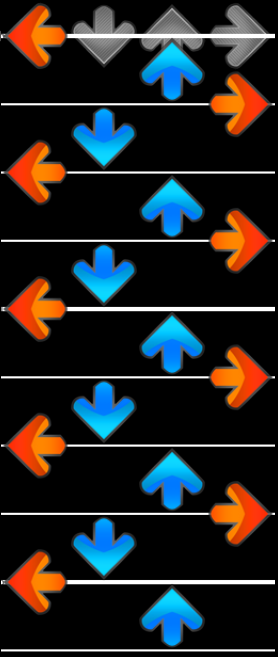
\includegraphics[width=0.17\textwidth]{result-2-spin.png} \\
		\small (a) Vanilla, $\mathcal{T}=4/3$. &
		\small (b) Crossovers, $\mathcal{T}=3/2$. &
		\small (c) Laterals, $\mathcal{T}=8/5$. &
		\small (d) 270s (irregular). &
		\small (e) Spins, $\mathcal{T}=2$.
	\end{tabular}
	\end{center}
	\caption{The turniest possible stepcharts.}
	\label{fig:sequences}
\end{figure*}

%%%%%%%%%%%%%%%%%%%%%%%%%%%%%%%%%%%%%%%%%%%%%%%%%%%%%%%%%%%%%%%%%%%%%%%%%%%%%%%%

\section{Existing Chart Analysis}

Of course, composing a stepchart of nothing but the theoretically-turniest patterns would be extremely tiresome (in more ways than one).
We turn our attention to existing ITG charts which were developed prior to this study, to investigate how much ITG players turn in the real world.
We processed every stepchart in our collection, which includes 70+ song packs.
Most well-known pack series from the ITG community are included, such as {\em Cirque}, {\em ITG}, {\em Mute Sims}, {\em Pendulum}, {\em r21*}, {\em SPEEDCOOOORE}, {\em The Legend of Zim}, and {\em Valex's Magical 4-Arrow Adventure}.

{\bf Limitations.}
Real-world stepcharts include many patterns not accounted for in our analysis. We did not expect much trouble from jumps and jacks, opting simply to ignore them and count the turns among the surrounding single-steps.
Footswitches and doublesteps, however, can foil this strategy, as our analysis will inadvertently begin stepping with feet inverted from where they should be.
Merely getting turned around is not a problem (computers don't have eyes), but the act of turning around involves some candle-steps, which could cause a footswitch-heavy chart to seem very spinny even though the proper footing would never make the player cross over at all.
Coping with these limitations is beyond the scope of our work, although we will highlight some experimental false-positives later.

\subsection{Results}

As shown in Figure~\ref{fig:distribution}, the vast majority of real-world stepcharts have average turniness between 0.6 and 1.0.
We don't really care about those.

\begin{figure}[t]
	\begin{center}
	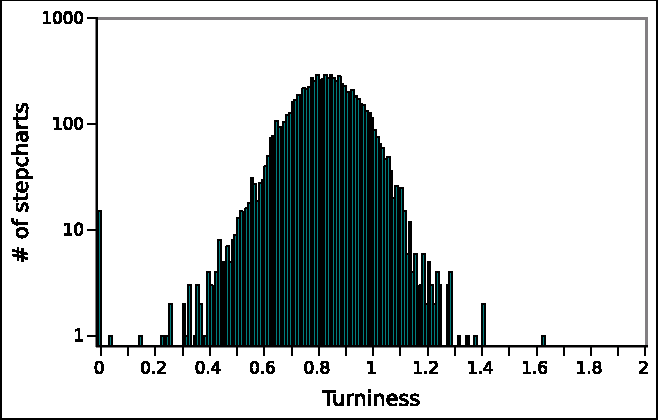
\includegraphics[width=0.48\textwidth]{realworld.pdf}
	\end{center}
	\caption{Distribution of turniness among 8,278 existing ITG charts.}
	\label{fig:distribution}
\end{figure}

{\bf The Least Turny Charts.}
16 charts in our collection have $\mathcal{T}=0$. Most of these are beginner charts, rated 2 or 3 feet and with no more than 100 steps. \cite{deltamax} stands out, as a 15-footer with 945 steps. God is that chart ever annoying.

Ignoring all beginner-difficulty and turn-free charts, the least turny stepchart is {\em Sick Dubstep Track} \cite{sickdubstep}, a 4-measure joke rated 6,482 feet, the majority of which is shown in Figure~\ref{fig:example}(a).


{\bf The Turniest Charts.}
No joker has yet dared to make the turniest possible chart (all spins), but one chart comes close.
Standing alone as the only chart turnier than 1.5 is the Easy 3 for {\em DO ME} \cite{dome}, which is mostly spins punctuated by a few breaks, as shown in Figure~\ref{fig:example}(d).
\cite{alanv} loves this chart.

Actually, 20 of the 30 turniest charts are all from DDR packs, most of which are Easies. Although DDR charts are known for being fairly crossovery in the upper ranges of difficulty, a close inspection of the easier charts will show that very little care was put in while writing them to avoid excessive double-stepping.
It's no wonder new ITG players, who used to play DDR, always double-step even when they don't need to. Sheesh, Konami.

Beyond these extreme examples, we are interested in some more normal charts people might actually like to play.
Table~\ref{tab:feets} shows the turniest charts of each level, for the most popular difficulty levels ranging from 7 to 17.
So, next time you want to work on your laterals or candles, you have me to thank!

Surprisingly, {\em BRILLIANT 2U (Orchestra-Groove)} \cite{brilliant2u} is full of 270s. I didn't think anybody ever put those in real charts.
Finally, an honourable mention goes to {\em Oedo Hop} \cite{oedo}, the 2nd turniest 7 (and 4th turniest chart overall!) with $\mathcal{T}=1.384$.
\cite{deltax} really likes that one so we had to mention it.

\begin{figure*}[t]
	\begin{center}
	\begin{tabular}{cccc}
		\hspace{-2em}
		\begin{tabular}{c}
		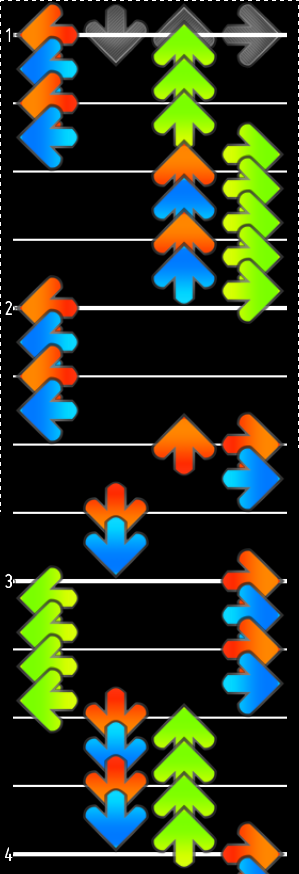
\includegraphics[width=0.18\textwidth]{sick-dubstep-track.png} \\
		\small
		\begin{tabular}{l}
			(a) {\em Sick Dubstep Track}, $\mathcal{T}=0.26$. \\
		The least turny non-trivial \\
		chart.\\
		\\
		\end{tabular}
		\end{tabular}
		&
		\hspace{-1.5em}
		\begin{tabular}{c}
		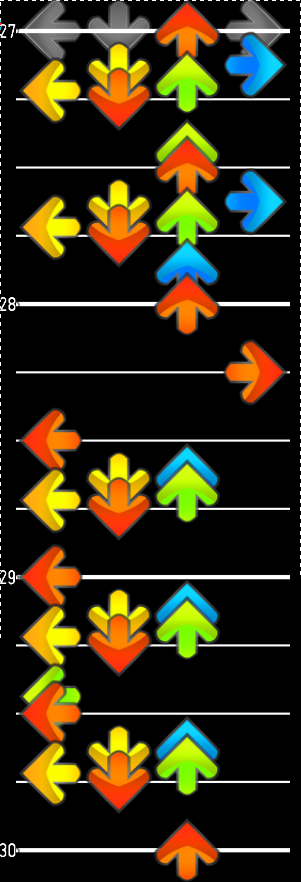
\includegraphics[width=0.18\textwidth]{mr-saxobeat.png} \\
		\small
		\begin{tabular}{l}
			(b) {\em Mr. Saxobeat}, $\mathcal{T}=1.04$. \\
		Look at all those candles! \\
		No wonder it was so hard \\
		for the author to pass.\\
		\end{tabular}
		\end{tabular}
		&
		\hspace{-1.5em}
		\begin{tabular}{c}
		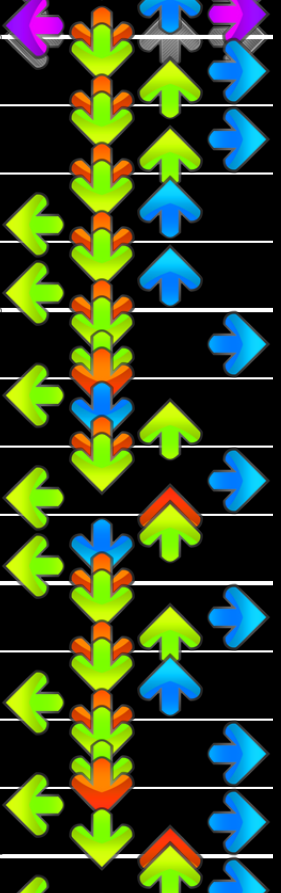
\includegraphics[width=0.185\textwidth]{flames.png} \\
		\small
		\begin{tabular}{l}
			(c) {\em Flames of the Sky}, $\mathcal{T}=1.04$. \\
			False-positive $\mathcal{T}$ from foot-\\
		switches. Actually faces $R$/$UR$/\\
		$U$/$UL$/$L$ the whole time.
		\end{tabular}
		\end{tabular}
		&
		\hspace{-1.5em}
		\begin{tabular}{c}
		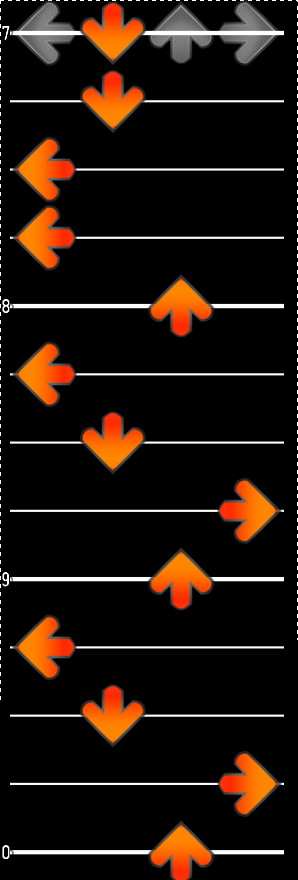
\includegraphics[width=0.18\textwidth]{do-me.png} \\
		\small
		\begin{tabular}{l}
			(d) {\em DO ME}, $\mathcal{T}=1.63$. \\
		I'll pass, thanks.\\
		\\
		\\
		\end{tabular}
		\end{tabular}
	\end{tabular}
	\end{center}
	\caption{Real-world ITG charts of varying degrees of turniness.}
	\label{fig:example}
\end{figure*}

\begin{table}[t]
	\begin{center}
		\small
	\begin{tabular}{r|l|l|c}
		Ft. & Name & Pack & $\mathcal{T}$ \\
		\hline
		7 & Trip Machine & DDR 1st & 1.407 \\
		%7 & Oedo Hop & r2112 & 1.38 \\
		%  & (honorable mention; way better chart) & & \\
		8 & Brilliant 2U (O-G) & DDR 2ndMIX & 1.347 \\
		9 & Hearts of Ice & In The Groove 3 & 1.127 \\
		10 & Visible Noise & In The Groove 2 & 1.188 \\
		11 & KKKKK Come On & r2112 & 1.145 \\
		12 & Winnipeg is Fucking Over & best of r21freak ii & 1.150 \\
		13 & Mr. Saxobeat (*) & Sexuality Violation 2 & 1.044 \\
		14 & Fancy Footwork ($\dagger$) & Cirque du Zeppelin & 1.026 \\
		15 & Flames of the Sky (*,$\dagger$) & Ft. Rapids VII &  1.037 \\
		16 & {\em (no 16 with $\mathcal{T}\ge 1$)} & - & - \\
		17 & Superluminal & Ft. Rapids VII & 1.058 \\
	\end{tabular}
	\end{center}
	\caption{The turniest existing stepcharts of each difficulty. Songs marked (*) are also shown in Figure~\ref{fig:example}. Songs marked ($\dagger$) are false-positives resulting from too many footswitches incorrectly analyzed as spins.}
	\label{tab:feets}
\end{table}

{\bf The Turniest Other Things.}
Although our analysis picked out a good many turny charts, any ITG player will inevitably get tired of playing the same ones over and over.
Hence, we are also interested in an aggregated turniness profile to show the average scores of many different stepcharts at once.
We computed average turninesses for stepcharts grouped {\em by pack} and {\em by step artist}.
Abbreviated results for the former are shown in Table~\ref{tab:pack} and for the latter in Table~\ref{tab:artist}.
For the sake of players who dislike turniness, we also list the lowest-scoring packs and artists in addition to the highest-scoring ones.

\begin{table}[t]
	\begin{center}
		\small
	\begin{tabular}{l|c|c}
		Song Pack & \# of Charts & Avg. $\mathcal{T}$ \\
		\hline
		Valex's Magical 4-Arrow Adventure 5 & 150 & 0.964 \\
		Valex's Magical 4-Arrow Adventure 4 & 170 & 0.956 \\
		Valex's Magical 4-Arrow Adventure 3 & 155 & 0.950 \\
		Valex's Magical 4-Arrow Adventure 7 & 150 & 0.937 \\
		Valex's Magical 4-Arrow Adventure 2 & 130 & 0.929 \\
		Valex's Magical 4-Arrow Adventure   & 95 & 0.919 \\
		Valex's Magical 4-Arrow Adventure 6 & 145 & 0.917 \\
		Subluminal & 16 & 0.906 \\
		The Legend of Zim 1 & 26 & 0.906 \\
		FoxyMix 5 & 30 & 0.901 \\
		FoxyMix 4 - Nuclear Overdrive & 68 & 0.899 \\ 
		Mute Sims 9 & 48 & 0.886 \\
		In The Groove Rebirth + & 147 & 0.881 \\
		StepMania 5 & 5 & 0.869 \\
		\multicolumn{3}{c}{\normalsize\dots} \\
		Stephcharts and Richarts & 81 & 0.770 \\
		Tachyon Delta & 32 & 0.769 \\
		Tachyon Alpha & 151 & 0.769 \\
		Sexuality Violation 2 & 219 & 0.766 \\
		TLOES Chapter 1 & 120 & 0.765 \\
		Fort Rapids V (12s-16s) r3 Final & 98 & 0.759 \\
		Noisiastreamz & 20 & 0.758 \\
		In The Groove & 331 & 0.754 \\
		Pendulum & 150 & 0.747 \\
		SPEEDCOOOORE 2 & 70 & 0.731 \\
		SPEEDCOOOORE & 47 & 0.709 \\
		The Legend of Zim 3 & 40 & 0.702 \\
		The Legend of Zim 4 & 44 & 0.701 \\
		The Legend of Zim 5 & 19 & 0.667 \\
	\end{tabular}
	\end{center}
	\caption{The turniest and least turny stepfile packs. Wow, great job Valex! Zim had a good thing going but has been slacking off recently.}
	\label{tab:pack}
\end{table}
\begin{table}[t]
	\begin{center}
		\small
	\begin{tabular}{l|c|c}
		Step Artist & \# of Charts & Avg. $\mathcal{T}$ \\
		\hline
		M. Emirzian & 25 & 0.981 \\
		sssmsm & 40 & 0.980 \\
		M. Calfin & 16 & 0.947 \\
		J. Berkowitz (Valex) & 1016 & 0.940 \\
		B. Dinh & 10 & 0.919 \\
		J. DeGarmo & 24 & 0.915 \\
		X. Ythar & 17 & 0.914 \\
		R. McKanna & 59 & 0.895 \\
		R. Woods & 18 & 0.892 \\
		Fraxtil & 23 & 0.880 \\
		\multicolumn{3}{c}{\normalsize\dots} \\
		I. Pyles & 175 & 0.754 \\
		P. Shanklin & 29 & 0.752 \\
		Gazebo & 355 & 0.751 \\
		zimlord & 199 & 0.750 \\
		C. Emirzian & 17 & 0.736 \\
		Mootz & 22 & 0.734 \\
		B. Abear & 27 & 0.729 \\
		Insane Steve & 41 & 0.718 \\
		Blazing & 15 & 0.696 \\
		C. Foy & 138 & 0.678 \\
	\end{tabular}
	\end{center}
	\caption{The turniest and least turny step authors. Only authors with 10 or more charts are included.}
	\label{tab:artist}
\end{table}


\section{Conclusion}


In conclusion, $LURR$ $DURR$!

%%%%%%%%%%%%%%%%%%%%%%%%%%%%%%%%%%%%%%%%%%%%%%%%%%%%%%%%%%%%%%%%%%%%%%%%%%%%%%%%

\appendix

\section{Linx}

Our analysis program can be found at \url{https://github.com/bblum/sigbovik/tree/master/itg/code}, and our full experimental data-set is available at \url{http://tinyurl.com/turniness}.

\section{Most turny patterns}

% TODO: figure out how to uniquify these.

\subsection{Vanilla}

Following are the most turny 18-step patterns that are totally vanilla, with turniness of 1.375. (Manual inspection reveals the true turniness to be 4/3.)

\noindent
URDULDURDULDURDULD
DRUDLUDRUDLUDRUDLU

\subsection{Crossovers}

Following are the most turny 18-step patterns that may include crossovers only, with turniness of 1.5.

\noindent
URDULDURDLDRULURDL
URDULDRDLUDRULURDL
URDULDRDLURULDURDL
URDULDRDLURULDRDLU
URDLDRUDLUDRULURDL
URDLDRUDLURULDURDL
URDLDRUDLURULDRDLU
URDLDRULURDULDURDL
URDLDRULURDULDRDLU
URDLDRULURDLDRUDLU
URDLDRULURDLDRULUR
URDLDRULURDLDRURDL
URDLDRULURDRULURDL
URDLDRURDLDRULURDL
URDRULURDLDRULURDL
DRUDLUDRULURDLDRUL
DRUDLURULDURDLDRUL
DRUDLURULDRDLUDRUL
DRUDLURULDRDLURULD
DRULURDULDURDLDRUL
DRULURDULDRDLUDRUL
DRULURDULDRDLURULD
DRULURDLDRUDLUDRUL
DRULURDLDRUDLURULD
DRULURDLDRULURDULD
DRULURDLDRULURDLDR
DRULURDLDRULURDRUL
DRULURDLDRURDLDRUL
DRULURDRULURDLDRUL
DRURDLDRULURDLDRUL
LUDRULURDLDRULURDL
LURULDURDLDRULURDL
LURULDRDLUDRULURDL
LURULDRDLURULDURDL
LURULDRDLURULDRDLU
LDURDLDRULURDLDRUL
LDRDLUDRULURDLDRUL
LDRDLURULDURDLDRUL
LDRDLURULDRDLUDRUL
LDRDLURULDRDLURULD

\subsection{Laterals}

Following are the most turny 18-step patterns that may include crossovers and laterals, with turniness of 1.625. (Manual inspection reveals the true turniness to be 8/5.)

\noindent
URDLDRULRDLURLDRUL
URDLRULDRDLURLDRUL
URDLRULDRLURDLDRUL
URDLRULDRLURDLRULD
DRULURDLRULDRLURDL
DRULRDLURULDRLURDL
DRULRDLURLDRULURDL
DRULRDLURLDRULRDLU
LURLDRULRDLURLDRUL
LDRLURDLRULDRLURDL

\subsection{270s}

Following are the most turny 18-step patterns that may include crossovers, laterals, and 270s, with turniness of 1.625.
(Manual inspection reveals irregularity; these streams exhibit no core pattern that can be repeated to retain the maximum turniness.)

\noindent
URDULDRLURDLRULDRU
URDLDRULURDLRULDRU
URDLDRULRDLURULDRU
URDLDRULRDLURLDRUL
URDLRULDURDLRULDRU
URDLRULDRDLURULDRU
URDLRULDRDLURLDRUL
URDLRULDRLURDULDRU
URDLRULDRLURDLDRUL
URDLRULDRLURDLRULD
DRUDLURLDRULRDLURD
DRULURDLDRULRDLURD
DRULURDLRULDRDLURD
DRULURDLRULDRLURDL
DRULRDLUDRULRDLURD
DRULRDLURULDRDLURD
DRULRDLURULDRLURDL
DRULRDLURLDRUDLURD
DRULRDLURLDRULURDL
DRULRDLURLDRULRDLU
LURULDRLURDLRULDRU
LURLDRULURDLRULDRU
LURLDRULRDLURULDRU
LURLDRULRDLURLDRUL \\
LDRDLURLDRULRDLURD
LDRLURDLDRULRDLURD
LDRLURDLRULDRDLURD
LDRLURDLRULDRLURDL

\subsection{Spins}

Following are the most turny 18-step patterns that may include any pattern, with turniness of 2.

\noindent
URDLURDLURDLURDLUR
DRULDRULDRULDRULDR
LURDLURDLURDLURDLU
LDRULDRULDRULDRULD

\bibliographystyle{abbrvnat}
\bibliography{citations}

\end{document}
